% !TeX spellcheck = en_US
\addscenariosection{1}{Campaign name}{Scenario name}{\images/title.png}

\begin{multicols*}{2}

\textbf{Author:} ...

\textbf{Source:} ...

\subsection*{\MakeUppercase{Scenario length}}

This scenario plays out over ... rounds.

\subsection*{\MakeUppercase{Player setup}}

\textbf{Faction:} ...

\textbf{Faction Hero:} ...

\textbf{Starting Resources:} \svg{gold} \svg{building_materials} \svg{valuables}

\textbf{Starting Income:} \svg{gold} \svg{building_materials} \svg{valuables}

\textbf{Starting Units:} \svg{bronze} \svg{silver} \svg{golden} \svg{azure}

\textbf{Town Buildings:} ...

\textbf{Bonus:} Choose one of the following options: 
\begin{itemize}
    \item ...
\end{itemize}

\subsection*{\MakeUppercase{AI hero setup}}

\textbf{Faction:} ...

\textbf{Enemy Army:} ...

\textbf{Enemy Deck:} ...

\textbf{Enemy Spell Deck:} ...

\textbf{Enemy Skills:} ...

\textbf{Special:} ...

\subsection*{\MakeUppercase{Map setup}}

Take the following Map tiles and arrange them as shown in the scenario map layout:

\textbf{X × Starting Map tile (I)}
\begin{itemize}
    \item ... additional constraints ...
\end{itemize}

\textbf{Y × Far Map tile (II-III)}

\textbf{Z × Near Map tile (IV-V)}

\subsection*{\MakeUppercase{Heroes placement}}

... describe how your and enemy heroes will be placed ...

\subsection*{\MakeUppercase{Additional rules}}

During this ``... faction ...'' campaign scenario, the following rules apply:

\begin{itemize}
    \item ...
\end{itemize}

\subsection*{\MakeUppercase{Win/lose conditions}}

\textbf{Win:}
\begin{itemize}
    \item ...
\end{itemize}

\textbf{Lose:}
\begin{itemize}
    \item ...
\end{itemize}

\subsection*{\MakeUppercase{Timed Events}}

\textbf{X$^{th}$ Round:}
\begin{itemize}
  \item ...
  \item ...
\end{itemize}

% IF THERE ARE OVERLAPPING EVENTS, FOLLOW BELOW STRUCTURE, IN CHRONOLOGICAL ORDER
%
% \textbf{7$^{th}$ and 8$^{th}$ Rounds:}
% \begin{itemize}
%   \item ...
% \end{itemize}
%
% \textbf{9$^{th}$ Round:}
% \begin{itemize}
%   \item Repeat Timed Events of Round 6.
% \end{itemize}
% 
% \textbf{10$^{th}$ Round:}
% \begin{itemize}
%   \item Repeat Timed Events of Rounds 7 and 8.
% \end{itemize}

\end{multicols*}

\newpage

% NOTE: The last page of scenario preparation should use 
% multicols instead of multicols* to create space for map.
% \begin{multicols}{2}
% ... your content that overflows to the second page ...
% \end{multicols}

% Uncomment and link a map image
% \vspace{3em}
% \begin{center}
%   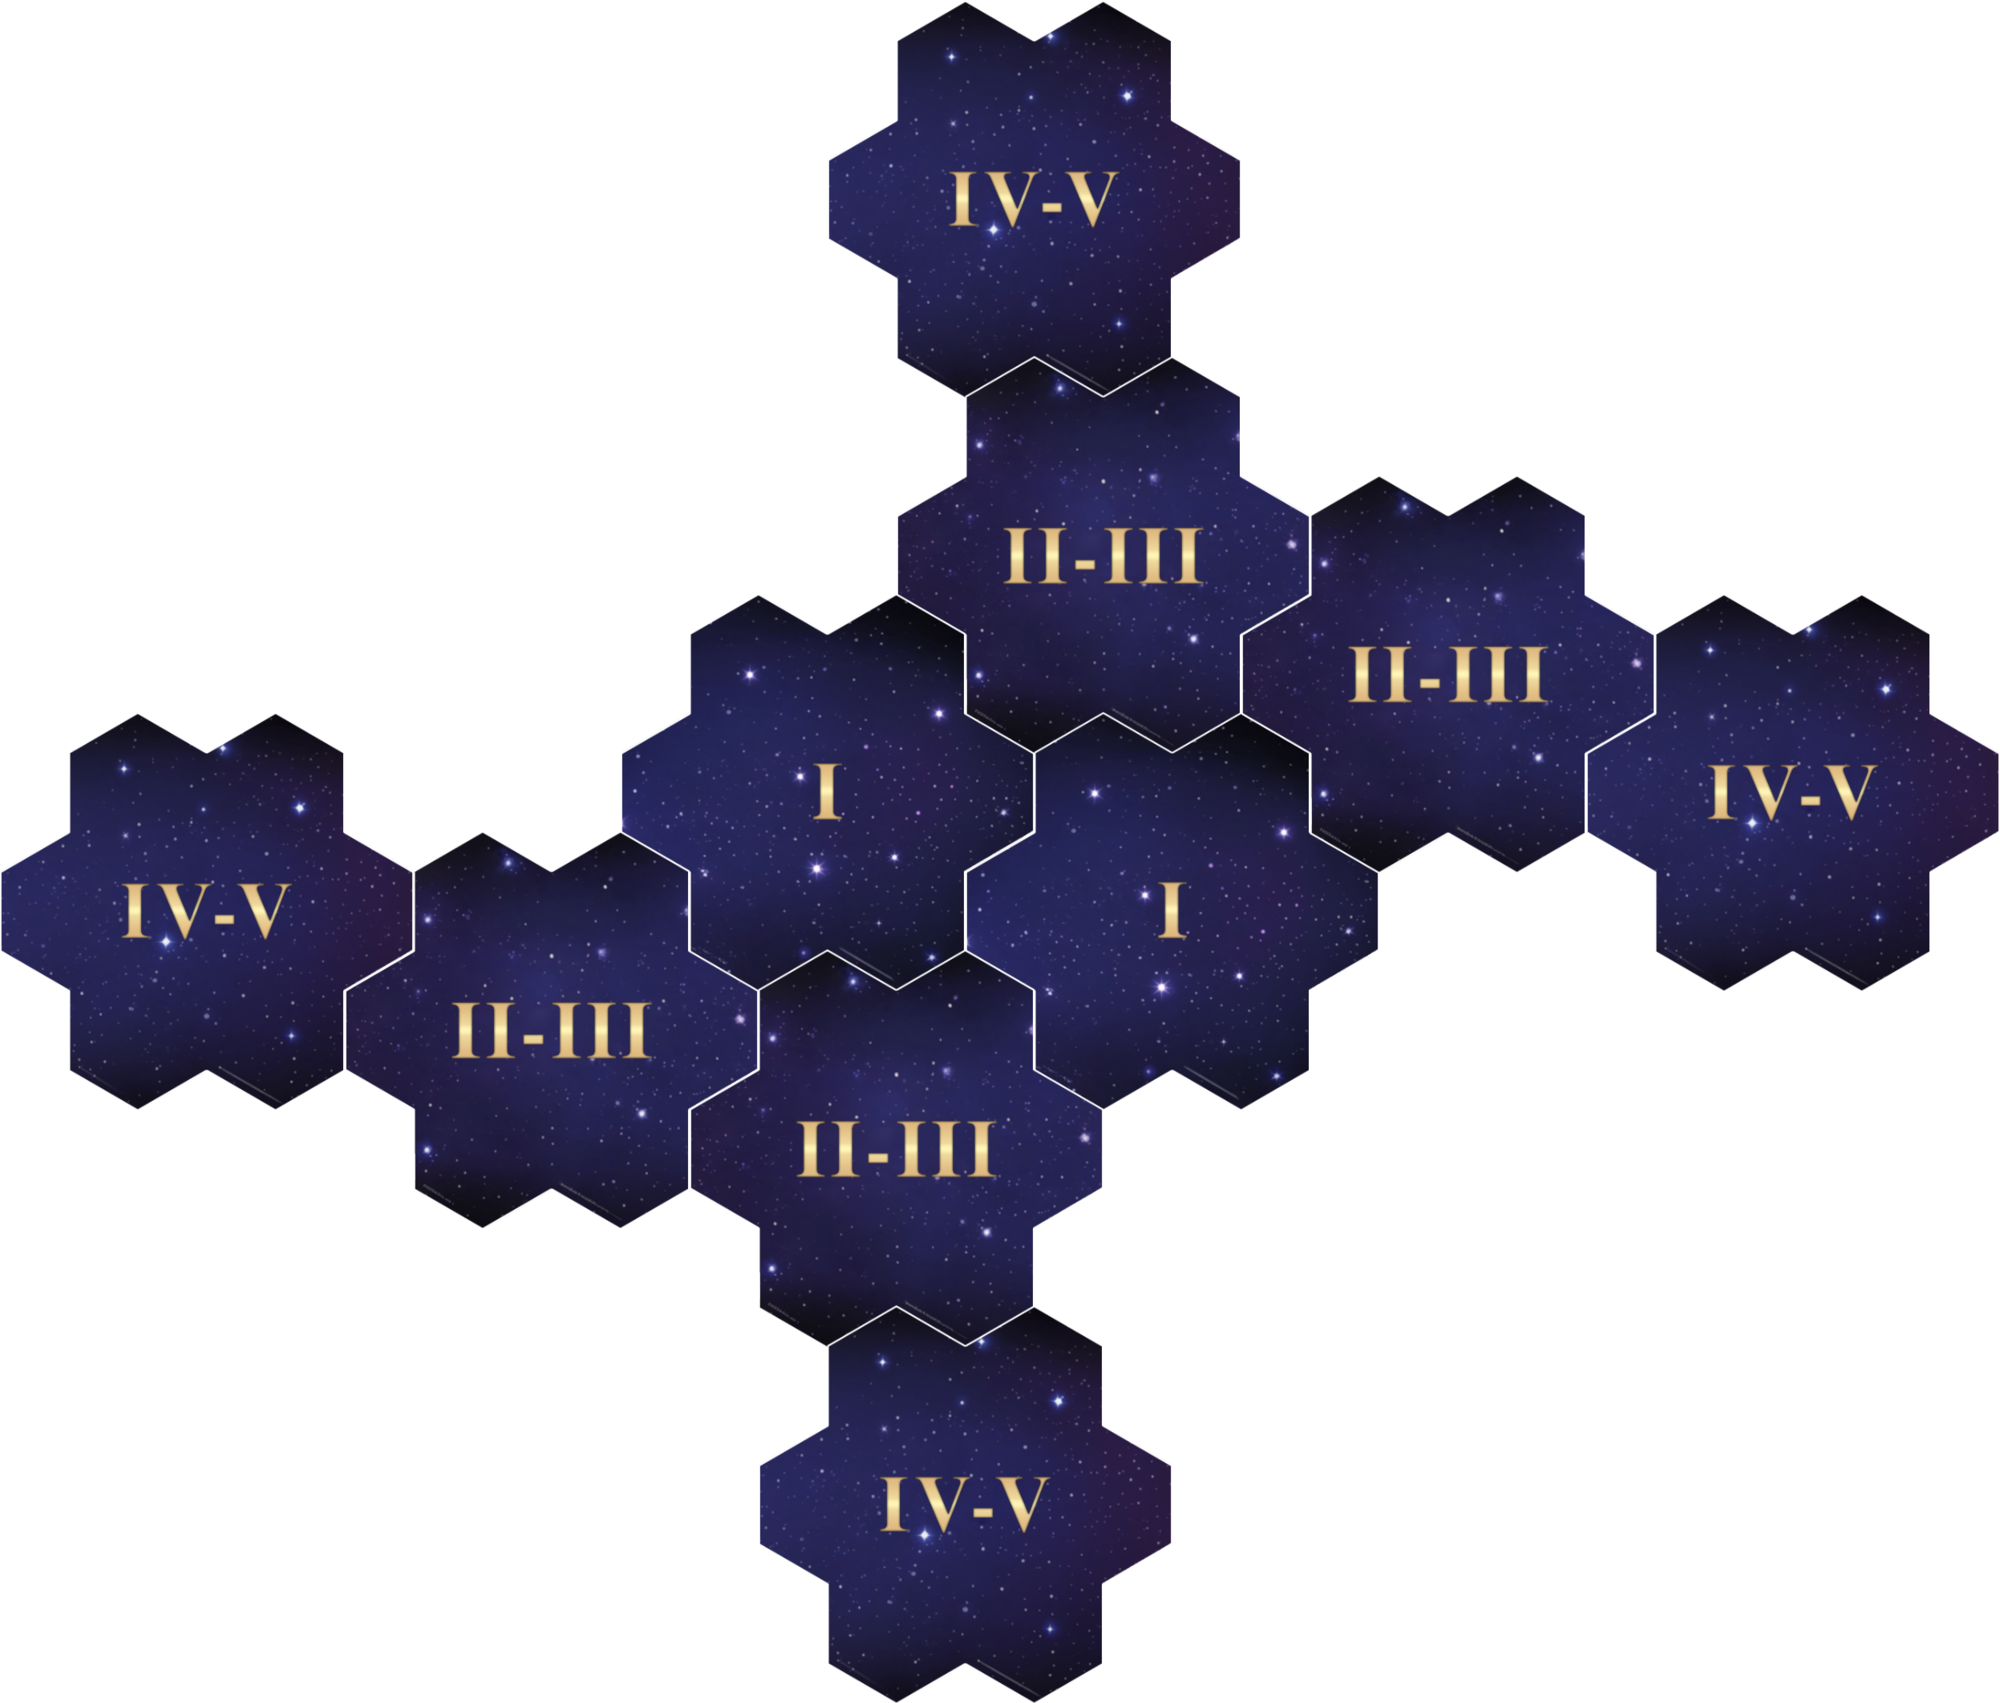
\includegraphics[width=0.6\paperwidth]{\_assets/maps/sentinels.png}
% \end{center}

\newpage

\begin{multicols*}{2}

\subsection*{\MakeUppercase{The story}}

... put your immersive story here ...

\end{multicols*}
